\documentclass[a4paper,10pt]{article}
\usepackage[utf8]{inputenc}
\usepackage[a4paper,
            bindingoffset=0.2in,
            left=1in,
            right=1in,
            top=1in,
            bottom=1in,
            footskip=.25in]{geometry}

%###############################################################################

%\input{~/layout/global_layout}


%###############################################################################

% packages begin

\usepackage[
  backend=biber,
  sortcites=true,
  style=alphabetic,
  eprint=true,
  backref=true
]{biblatex}
\addbibresource{bibliographie.bib}
\usepackage[acronym]{glossaries}

\usepackage{euscript}[mathcal]
% e.g. \mathcal{A} for fancy letters in mathmode
\usepackage{amsmath,amssymb,amstext,amsthm}

\usepackage{mdframed}
\newmdtheoremenv[nobreak=true]{problem}{Problem}[subsection]
\newmdtheoremenv[nobreak=true]{claim}{Claim}[subsection]
\newtheorem{definition}{Definition}[subsection]
\newtheorem{lemma}{Lemma}[claim]
\newtheorem{plemma}{Lemma}[problem]

\usepackage{mathtools}
\DeclarePairedDelimiter\ceil{\lceil}{\rceil}
\DeclarePairedDelimiter\floor{\lfloor}{\rfloor}

\usepackage{enumerate}
\usepackage[pdftex]{graphicx}
\usepackage{subcaption}
% 'draft' für schnelleres rendern mitübergeben -> [pdftex, draft]
% dadruch wird nicht das bild mitgerendered, sondern nur ein kasten mit bildname -> schont ressourcen

\usepackage{hyperref}

\usepackage{tikz}
\usetikzlibrary{arrows,automata,matrix,positioning,shapes}

% for adding non-formatted text to include source-code
\usepackage{listings}
\lstset{language=Python,basicstyle=\footnotesize}
% z.B.:
% \lstinputlisting{source_filename.py}
% \lstinputlisting[lanugage=Python, firstline=37, lastline=45]{source_filename.py}
%
% oder
%
% \begin{lstlisting}[frame=single]
% CODE HERE
%\end{lstlisting}
\usepackage{algorithm}
\usepackage{algpseudocode}

\usepackage{wasysym}

\usepackage{titling}
\usepackage{titlesec}
\usepackage[nocheck]{fancyhdr}
\usepackage{lastpage}
\usepackage{svg}

\usepackage{kantlipsum}
\usepackage[colorinlistoftodos,prependcaption,textsize=tiny]{todonotes}

% packages end
%###############################################################################

\pretitle{% add some rules
  \begin{center}
    \LARGE\bfseries
} %, make the fonts bigger, make the title (only) bold
\posttitle{%
  \end{center}%
  %\vskip .75em plus .25em minus .25em% increase the vertical spacing a bit, make this particular glue stretchier
}
\predate{%
  \begin{center}
    \normalsize
}
\postdate{%
  \end{center}%
}

\titleformat*{\section}{\Large\bfseries}
\titleformat*{\subsection}{\large\bfseries}
\titleformat*{\subsubsection}{\normalsize\bfseries}

\titleformat*{\paragraph}{\Large\bfseries}
\titleformat*{\subparagraph}{\large\bfseries}

%###############################################################################

\pagestyle{fancy}
\fancyhf{}
% l=left, c=center, r=right; e=even_pagenumber, o=odd_pagenumber; h=header, f=footer
% example: [lh] -> left header, [lof,ref] -> fotter left when odd, right when even
%\fancyhf[lh]{}
%\fancyhf[ch]{}
%\fancyhf[rh]{}
%\fancyhf[lf]{}
\fancyhf[cf]{\footnotesize Page \thepage\ of \pageref*{LastPage}}
%\fancyhf[rf]{}
\renewcommand{\headrule}{} % removes horizontal header line

% Fotter options for first page

\fancypagestyle{firstpagestyle}{
  \renewcommand{\thedate}{\textmd{}} % removes horizontal header line
  \fancyhf{}
  \fancyhf[lh]{\ttfamily M.Sc. Computer Science\\KTH Royal Institute of Technology}
  \fancyhf[rh]{\ttfamily Period 4\\\today}
  \fancyfoot[C]{\footnotesize Page \thepage\ of \pageref*{LastPage}}
  \renewcommand{\headrule}{} % removes horizontal header line
}
%###############################################################################

\newcommand\extrafootertext[1]{%
    \bgroup
    \renewcommand\thefootnote{\fnsymbol{footnote}}%
    \renewcommand\thempfootnote{\fnsymbol{mpfootnote}}%
    \footnotetext[0]{#1}%
    \egroup
}

%###############################################################################

\title{
  \normalsize{DD2356 VT25 Methods in}\\
  \normalsize{High Performance Computing}\\
  \large{Assignment 2}
}
\author{
  \small Rishi Vijayvargiya\textsuperscript{\textdagger}\\[-0.75ex]
%  \footnotesize\texttt{MN: }\\[-1ex]
  \scriptsize\texttt{rishiv@kth.se}
  \and
  \small Paul Mayer\textsuperscript{\textdagger}\\[-0.75ex]
%  \footnotesize\texttt{MN: }\\[-1ex]
  \scriptsize\texttt{pmayer@kth.se}
  \and
  \small Lennard Herud \textsuperscript{\textdagger}\\[-0.75ex]
%  \footnotesize\texttt{MN: }\\[-1ex]
  \scriptsize\texttt{herud@kth.se}
}
\date{}

%###############################################################################
% define Commands

\newcommand{\N}{\mathbb{N}}
\newcommand{\R}{\mathbb{R}}
\newcommand{\Z}{\mathbb{Z}}
\newcommand{\I}{\mathbb{I}}

\newcommand{\E}{\mathbb{E}}
\newcommand{\Prob}{\mathbb{P}}

\renewcommand{\epsilon}{\varepsilon}

%###############################################################################
\makeatletter
\renewcommand*{\@fnsymbol}[1]{\ensuremath{\ifcase#1\or \dagger\or \ddagger\or
   \mathsection\or \mathparagraph\or \|\or **\or \dagger\dagger
   \or \ddagger\ddagger \else\@ctrerr\fi}}
\makeatother
%###############################################################################

\begin{document}
\maketitle
\extrafootertext{\textsuperscript{\textdagger}Authors made equal contribution to the project}
\thispagestyle{firstpagestyle}

\listoftodos
\vspace{1em}

% content begin
%

\section*{Prefix}
The code for our project can be found at this location: \url{https://github.com/paulmyr/DD2356-MethodsHPC/tree/master/2_hpc_arch_perf_model}. 

\tableofcontents
\newpage


\section{}
\todo[inline]{Check headers}



\section{Exercise 1: Supercomputer Architecture with hwloc}
We first allocated a compute node using the following command: 
\begin{lstlisting}[language=bash,basicstyle=\ttfamily]
salloc -t 00:30:00 --nodes 1 --ntasks-per-node 128 --cpus-per-task 1 -A edu25.DD2356 -p shared
\end{lstlisting}

We retreive the Architecture using \verb|hwloc-ls --of svg > topology.svg| on the allocated node and then copying the file from the cluster to our repository using the securecopy \verb|scp| command. The resulting graphical representation can be seen in the repository \href{https://github.com/paulmyr/DD2356-MethodsHPC/blob/master/2_hpc_arch_perf_model/exercise1/topology.svg}{here}.
% \begin{figure}
 % \includesvg[width=\textwidth]{img/topology.svg}
%  \caption{Dardel Architecture}
 % \label{DardelArchitectureFigure}
% \end{figure}

We can see the following structure:
\begin{enumerate}
  \item Two NUMA nodes
  \item 16 CPU Sockets per node \todo{recheck}
  \item 4 CPU cores per Socket
\end{enumerate}
The cache per core consists of a $32 KB$ L1 instruction cache and a $32 KB$ L1 data cache, followed by a $512 KB$ L2 cache. The $16 MB$ L3 Cache is allocated per socket and thus shared between 4 CPU cores.

\todo{Document how memory is organized across NUMA nodes and how this affects performance.}
\todo{Specify 2 scenarios where memory locality influences execution time and resource efficiency.}
\todo{Contrast Dardel’s architecture with Top 5 supercomputers and discuss its implications for workload execution.}

\section{Exercise 2: Roofline Model}
x - axis: AI (arithmetic complexity) -> FLOPs / Byte
Here: Bytes is moved from main memory (especially read access).
Classify AI in O notation: O(1) very far to the left in roofline model
O(n) is far to the right in the roofline model!
Depends strongly on cache misses!
\todo{How to build the roofline model? What should the array size in stream benchmark be? Using 200mil causes errors during compilation. The default size seems too small according to comments in the code}
MEM/BW -> using stream line code to compute this line

To rank an application in the roofline model, one needs to determine the BYTE in AI.
For this one can use perf.
-> What hardware counter to use for this (we want to see cache misses)?

1) Query list of events that can be measured on a specific hardware
2) Select events that are related to cache misses, e.g. L2 cache misses.

-> What options do you have to link cache misses to parts of code? (out of scope of this lecture)

Note: On dardel: Linaro-forge installed (gperf not available because of missing sudo privileges).


\todo{How to establish the peak compute using the information of the processor?}
- FLOPs/sec limited given by the core (Hardware limit -> higher is never achievable)


\section{Exercise 3: Modeling Sparse Matrix-Vector Multiply}

\section{Exercise 4: Measure the Performance with Perf}
\subsection{Matrix Multiply}
\label{sec:matrix_multiply}
We created files \verb|matrix_multiply.c| and \verb|matrix_multiply_opt.c|, which were the default and optimized versions of the algorithm provided, respectively. We used the follogin \verb|salloc| command to allocate resources: 

\begin{lstlisting}[language=bash,basicstyle=\ttfamily]
salloc -t 00:30:00 --nodes 1  -A edu25.DD2356 -p shared
\end{lstlisting}
Since no \verb|--cpus-per-task| argument was provided, we believe that the default value of 1 was used. Additionally, since no \verb|-n| flag was provided either, we believe that the code was execute on 1 core. 

Compiling using the provided commands, we then executed \verb|perf| using the following command: 
\begin{lstlisting}[language=bash,basicstyle=\tiny\ttfamily]
srun -n 1 perf stat -e instructions,cycles,L1-dcache-load-misses,L1-dcache-loads ./matrix_multiply.out
\end{lstlisting}
The same thing was done for the optimized version. We varied \verb|MSIZE| manually, recompiled, and then re-executed the commands above for the different \verb|MSIZE| values. 
Doing so, we obtained the following table (for \textit{Elapsed time}, we record the values obtained from \verb|perf| and not the one produced by the algorithm) 
\begin{table}[h!]
\centering
\begin{tabular}{|c|p{2.5cm}|p{2.5cm}|p{2.5cm}|p{2.5cm}|}
\hline
\textbf{Event Name} & \textbf{Naive (MSIZE 64)} & \textbf{Optimized (MSIZE 64)} & \textbf{Naive (MSIZE 1000)} & \textbf{Optimized (MSIZE 1000)} \\
\hline
\textbf{Elapsed time (sec)} & 0.008982713 & 0.008476052 & 17.968526050 & 1.685069089 \\
\hline
\textbf{Instructions per cycle} & 1.16 & 1.28 & 0.58 & 2.17 \\
\hline
\textbf{L1 cache miss ratio} & 0.1817 & 0.0610 & 0.5618 & 0.1649 \\
\hline
\textbf{L1 cache miss rate PTI} & 101.5736 & 26.5007 & 400.6424 & 131.9917  \\
\hline
\end{tabular}
\caption{Perf Stats for Default and Optimized Matrix-Multiply}
\end{table}
The raw outputs for the different values of \verb|MSIZE| for the \verb|matrix_multiply.out| and \verb|matrix_multiply_opt.out| binaries can be found in the file \verb|matrix_multiply_outputs.txt| in the repository \href{https://github.com/paulmyr/DD2356-MethodsHPC/blob/master/2_hpc_arch_perf_model/exercise4/matrix_multiply_outputs.txt}{here}. For the \verb|L1 cache miss ratio| and the \verb|L1 cache miss rate PTI|, we used the formulas \href{https://canvas.kth.se/courses/53216/pages/tutorial-the-perf-tool?module_item_id=1067474}{here}.

From the experiment, we believe it is clear to see that the performance of the \verb|matrix_multiply| operation seems to be most affected by L1 cache misses. For the same \verb|MSIZE|, the higher the L1 cache misses, the lower the instructions per clock cycle, which leads to higher elapsed time and thus lower performance of the implementation. For both values of \verb|MSIZE|, the optimized version has fewer L1 cache misses and is thus more efficient.  

This demonstrates that the optimization, which focuses on using smaller physical strides when accessing \verb|matrix_a| and \verb|matrix_b| instead of iterating through columns of \verb|matrix_b|, is effective in lowering the L1 cache misses and making the algorithm more nimble and efficient. 

\subsection{Matrix Transpose}
\label{sec:matrix_transpose}
We created the file \verb|transpose.c| and compiled the program into 3 different binaries using the following command: 
\begin{lstlisting}[language=bash,basicstyle=\ttfamily]
cc -O2 -o transpose_n{grid_size}.out transpose.c
\end{lstlisting}
Here, the \verb|grid_size| depended on the size of \verb|N| required in the handout. Thus, it varied from 64 to 128 to 2048. 

We allocated compute nodes using the same \verb|salloc| command described for matrix multiplication. Finally, we ran each of the compiled binaries using the following \verb|srun| command: 
\begin{lstlisting}[language=bash,basicstyle=\tiny\ttfamily]
srun -n 1 perf stat -e instructions,cycles,L1-dcache-load-misses,L1-dcache-loads ./transpose_n{grid_size}.out
\end{lstlisting}
With this, we obtained the following outputs (\textit{Elapsed time} was recorded based on the output in \verb|perf|, not on the one produced by the program)
\begin{table}[h!]
\centering
\begin{tabular}{|c|p{2.5cm}|p{2.5cm}|p{2.5cm}|}
\hline
\textbf{Event Name} & \textbf{N 64} & \textbf{N 128} & \textbf{N 2048}  \\
\hline
\textbf{Elapsed time (sec)} & 0.040026827 & 0.008985869 & 35.493702241  \\
\hline
\textbf{Bandwidth / Rate} & 2.50e+04 MB/s & 6.94e+03 MB/s & 9.48e+01 MB/s \\
\hline
\textbf{Instructions per cycle} & 1.38 & 0.91 & 0.01 \\ 
\hline
\textbf{L1 cache miss ratio} & 0.0509 & 0.1683 & 0.2033 \\
\hline
\textbf{L1 cache miss rate PTI} & 23.7404 & 175.4544 & 3351.8774  \\
\hline
\end{tabular}
\caption{Perf Stats for Default and Optimized Matrix-Multiply}
\end{table}

Similar to the \ref{sec:matrix_multiply} analysis, we see that higher L1 cache misses lead to lower instructions per cycle and bandwidth. The elapsed time can be misleading in analysis here, since we have only one implementation, and higher values of \verb|N| will have more operations to perform, and thus a higher elapsed time for higher \verb|N| values could be expected. However, the bandwidth and instructions per cycle being lower for higher values of \verb|N| can be directly tied to the L1 cache miss ratios (as these are all unitary values). In short, the higher the L1 cache miss ratio for a run of the algorithm, the less efficient that run seems to be. 

\todo{Write 2-3 sentences on using cache-aware and cache-oblivious versions of the algorithm for matrix transpose}.

\section{Bonus: Network Latency \& Bandwidth Analysis with MPI Ping-Pong}
\subsection{Modifications to the Code}
There were some issues encountered in the provided code for \verb|mpi_ping_pong.c| file. 
\begin{itemize}
\item \verb|d| to \verb|lu| conversion when printing bytes: The original code gave a warning when compiled using \verb|cc mpi_ping_pong.c -o mpi_ping_pong|. \\
\item \verb|fflush(stdout)| immediately after printing information: As highlighted in the \href{https://canvas.kth.se/courses/53216/discussion_topics/456480}{discussion forum}, the code did not seem to terminate. Thus, adding \verb|fflush| statements after \verb|printf|s ensured that we get the output in this case. \textit{(Note: There was an answer provided by a student w.r.t modifying the code to ensure termination, but that did not seem to resolve the issue either. The student provided their entire modified code in the follow-up, but we did not use that version as we weren't sure if that matched with the semantics of the original code. Thus, we are not reporting the runtimes of the student-modified code here)}. 
\end{itemize}
The modified file can be found \href{https://github.com/paulmyr/DD2356-MethodsHPC/blob/master/2_hpc_arch_perf_model/bonus/mpi_ping_pong.c}{here}.

\subsection{Compiling, Allocating Nodes, and Running}
We allocated 2 different nodes, with 1 task per node, using the following command: 
\begin{lstlisting}[language=bash,basicstyle=\tiny\ttfamily]
salloc -t 00:30:00 --nodes 2 --ntasks-per-node 1 --cpus-per-task 1 -A edu25.DD2356 -p shared 
\end{lstlisting}
For compiling the file, we used the following command mentioned earlier: 
\begin{lstlisting}[language=bash,basicstyle=\ttfamily]
cc mpi_ping_pong.c -o mpi_ping_pong
\end{lstlisting}
Finally, to run the program, we used the following command provided in the handout: 
\begin{lstlisting}[language=bash,basicstyle=\ttfamily]
srun -N2 --ntasks=2 ./mpi_ping_pong
\end{lstlisting}

\subsection{Results}
The default code in \verb|mpi_ping_pong.c| only allowed \verb|size| to be atmost 1024 in the main loop. With this confirguration, apart from the very first send-receive interaction, the RTT for the other interactions seems to be relatively constant (the downward trend below can largely be attributed to the incredibly high RTT for the first interaction)

  \begin{figure}[H]
    \centering
    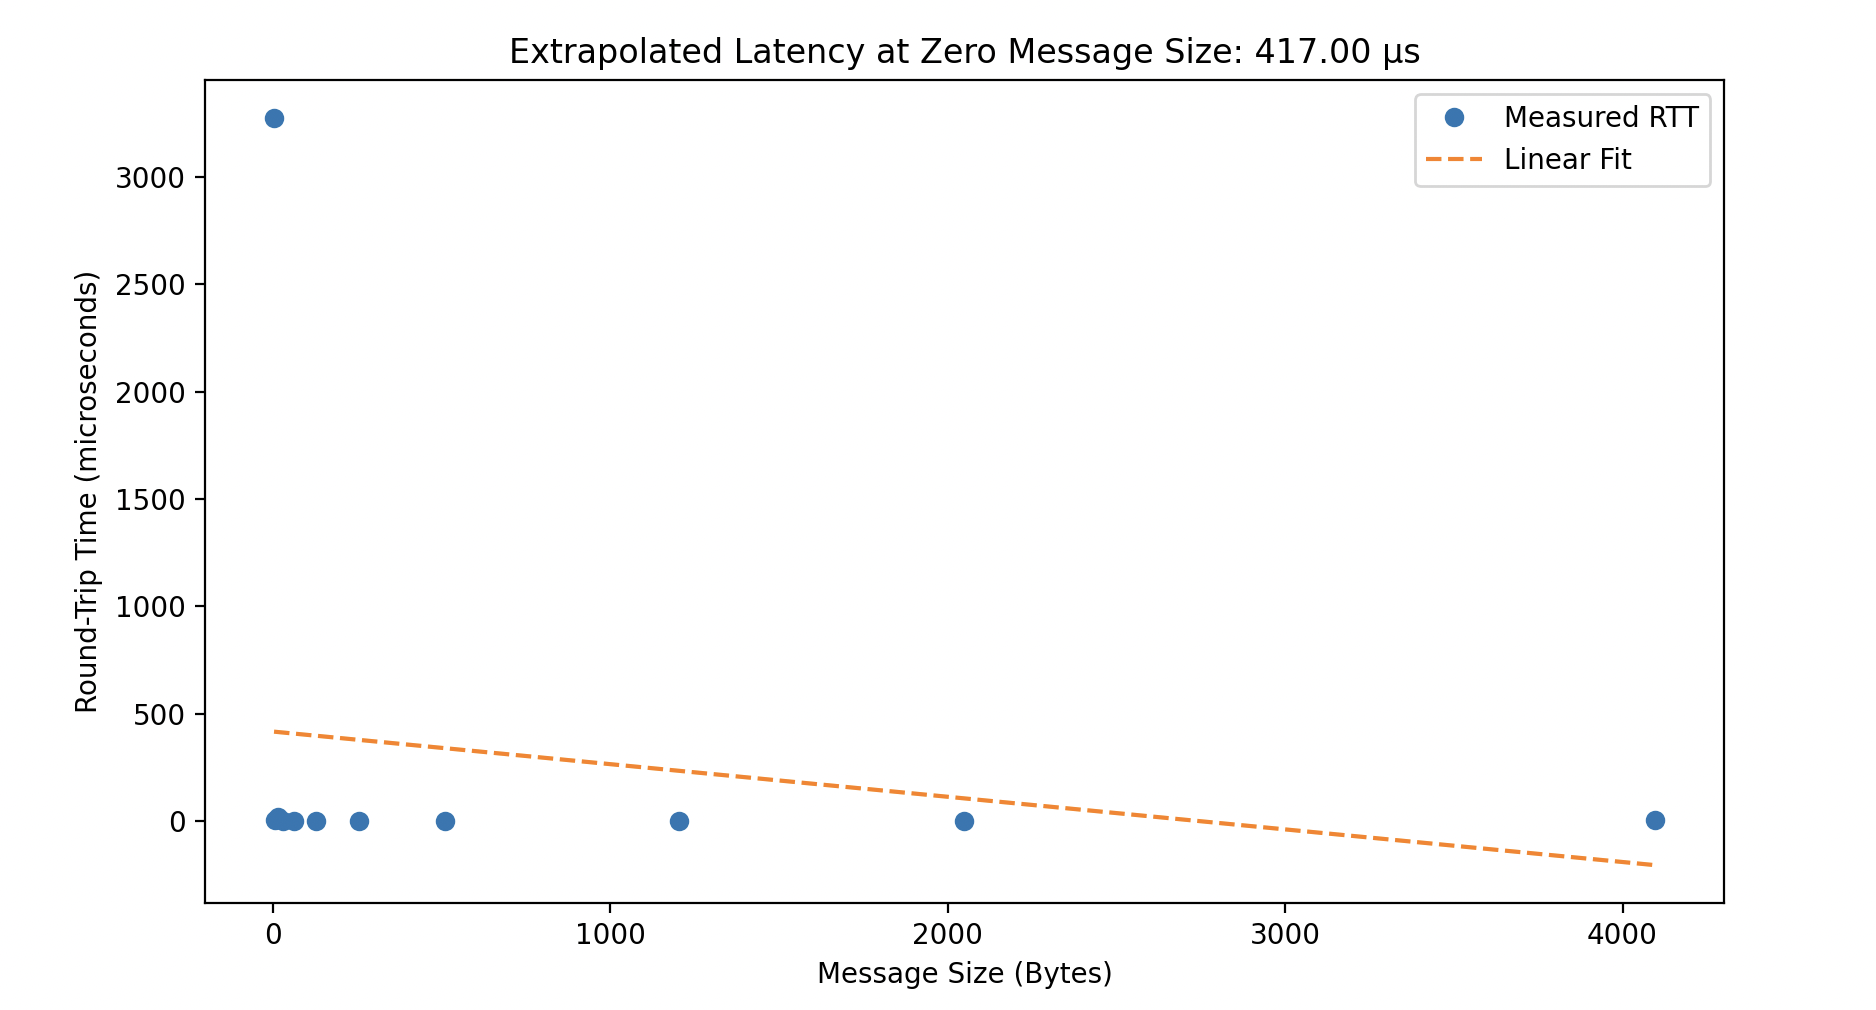
\includegraphics[width=0.9\textwidth]{img/bonus_lim1024}
    \caption{RTT Times (default limit)}
    \label{fig:bonus_rtt_default}
  \end{figure}
  
The graph of the output above was produced using the provided python plotting script, which can be found \href{https://github.com/paulmyr/DD2356-MethodsHPC/blob/master/2_hpc_arch_perf_model/bonus/graph_latency.py}{here}

We believe that the first interaction has a very high RTT because of the time required to setup the initial infrastructure that will be used for the rest of the communication. On the recommendation of Professor Peng, we increased the \verb|size| limit (\href{https://github.com/paulmyr/DD2356-MethodsHPC/blob/master/2_hpc_arch_perf_model/bonus/mpi_ping_pong.c#L14}{here}) to see some increase in the RTT to 65536 instead of 1024. With this setup, however, we started receiving segmentation faults after either 16384 bytes or 32768 bytes (this seems to vary on a run-by-run basis). This means that after \verb|size| reaches $32768 / 4 = 4096$ (since the printed size is multiplied with 4), there seems to be an error with the code which causes a segmentation fault. 

We did not attempt to spend time fixing the issue as we haven't yet been introduced to MPI in the course and because we did not wish to change the semantics of the original code. However, even with the output that was produced, we were able to see a gradual increasing trend in RTT as the size increases, as illustrated in the graph below (for a run which failed after 32768 bytes of data being sent). 

  \begin{figure}[H]
    \centering
    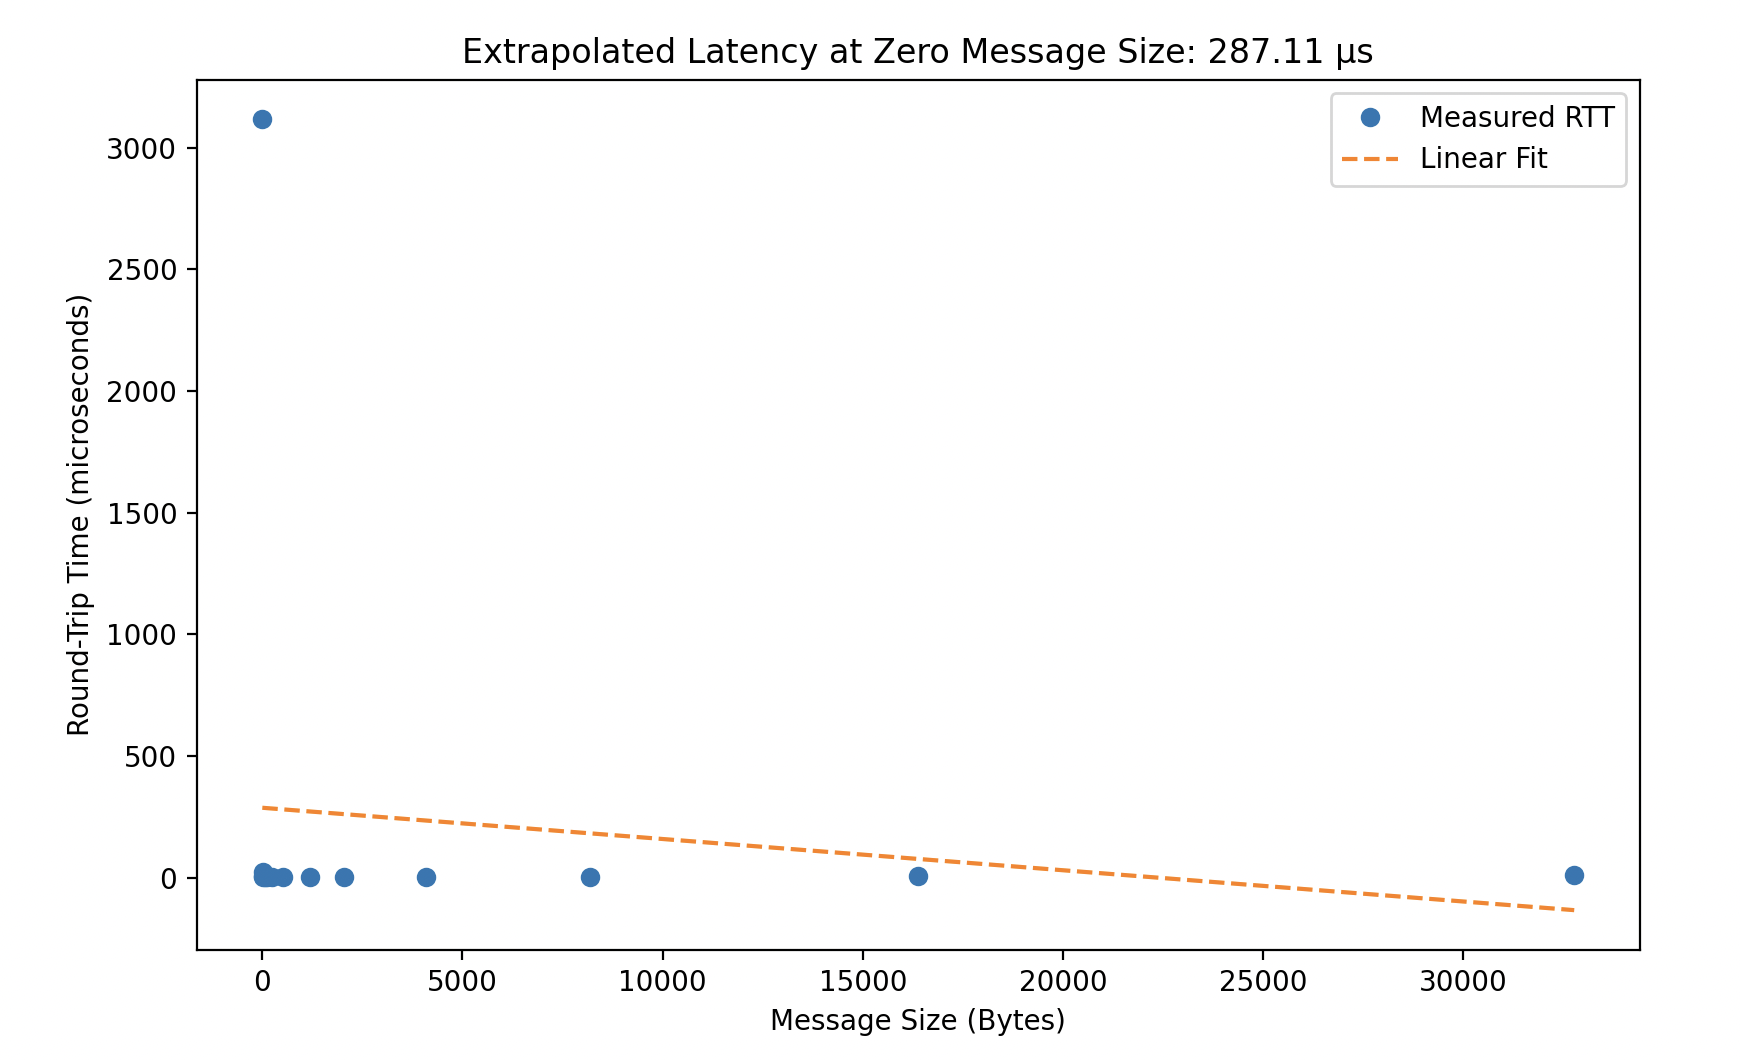
\includegraphics[width=0.9\textwidth]{img/bonus_lim65536}
    \caption{RTT Times (size limit changed to 65536)}
    \label{fig:bonus_rtt_large}
  \end{figure}

The textual outputs for the 2 runs plotted above can be found in the \verb|outputs.txt| file \href{https://github.com/paulmyr/DD2356-MethodsHPC/blob/master/2_hpc_arch_perf_model/bonus/outputs.txt}{here}

The incredibly high RTT time for the first send-receive interaction seems to makes it difficult to draw conclusions from the graph that can be drawn from the textual output. Thus, if we omit the plotting of the first recorded interaction, we obtain the following graph (\textit{Note: it is not clear to us if the extrapolated time at 0 message size recorded in the graph below serves a purpose any longer, but we still include the default output of the plotting script given the messages sizes and RTT without the first interaction})

  \begin{figure}[H]
    \centering
    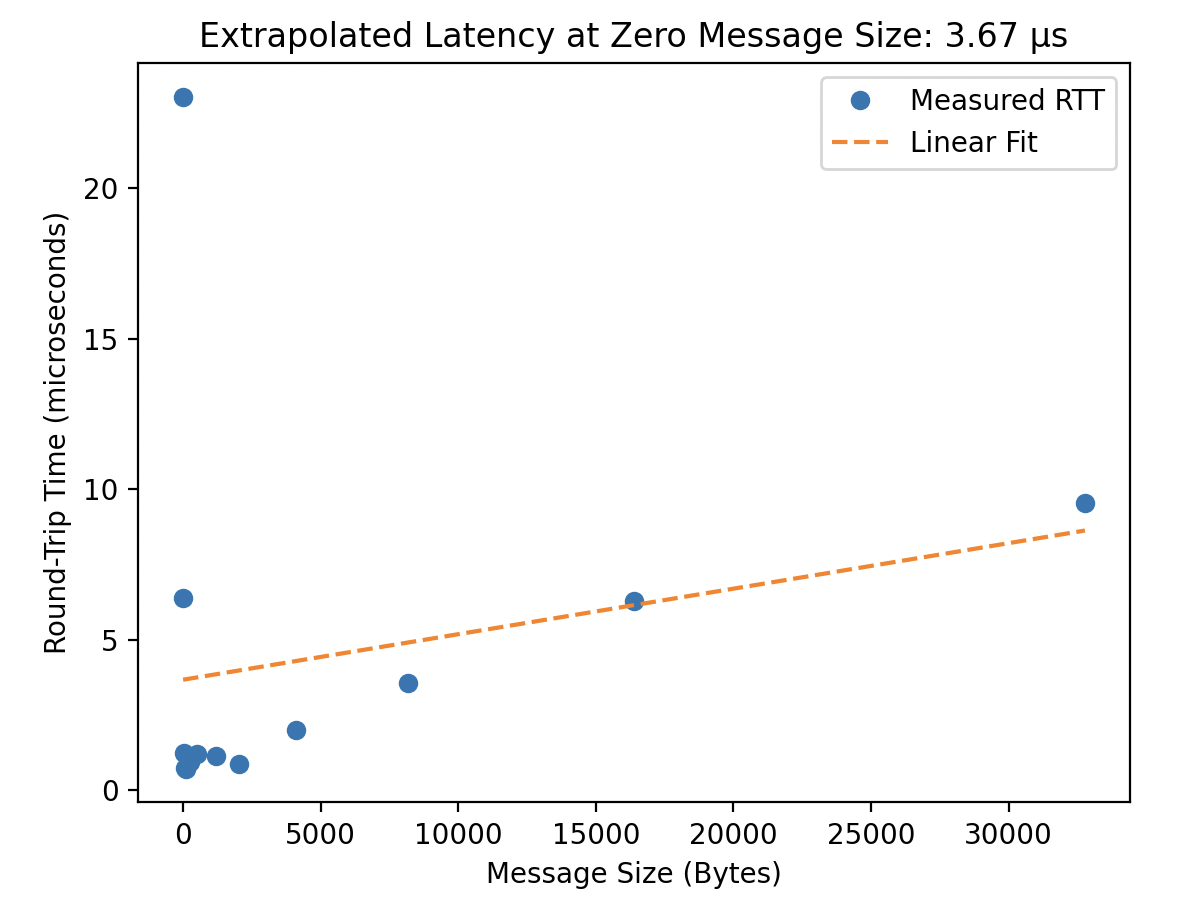
\includegraphics[width=0.9\textwidth]{img/bonus_large_pattern}
    \caption{RTT Times (omitting outlier RTT in first interaction)}
    \label{fig:bonus_rtt_pattern}
  \end{figure}


Through this, we can clearly see the following pattern in both the textual outputs and the graph: The RTT for the very first communication is an outlier, likely because of the initial cost of the send-receive infrastructue setup. After the first transmission, the RTT seems to be relatively constant for the next few sizes (except for a slight jump at 16 bytes). However, after a certain limit (in this case, it seems to be 4096 bytes of data sent), there seems to be an increase in RTT for each successive size. While the assignment does not ask for an explanation of these results, we believe this increase in RTT with increase in sizes after a certain point could be attributed to the multiple chunks in which data needs to be sent across nodes by MPI for larger sizes. 



% content end
%###############################################################################

% \printbibliography

\end{document}
